% textidote: ignore begin
\section{Architectural design}\label{sec:architectural-design}
% textidote: ignore end

When creating a structured system, it is important to consider the design of the system.
The architectural design is the first step in the design process.
In this section the group will present the criteria they have chosen to focus on and the architecture diagram of the
backend of the system.

\subsection{Criterion}\label{subsec:criterion}

The criterion is a list of requirements for the design of the system.
It shows the fields of the system that the group has focuses on.
The specific criteria were taken from a list of standard criteria for software systems~\cite[180]{mathiassen2018}. 

\begin{table}[H]
    \centering
    \resizebox{\columnwidth}{!}{%
        \begin{tabular}{ccccc}
            \toprule
            \textbf{Criterion} & \textbf{Very important} & \textbf{Important} &
            \textbf{Less important} & \textbf{Irrelevant} \\ \midrule
            Usable & X \\ \midrule
            Secure & & X \\ \midrule
            Efficient & & & & X \\ \midrule
            Correct & X \\ \midrule
            Reliable & & X \\ \midrule
            Maintainable & & & X \\ \midrule
            Testable & & & X \\ \midrule
            Flexible & & & X \\ \midrule
            Comprehensible & & X \\ \midrule
            Reusable & & & & X \\ \midrule
            Portable & & & & X \\ \midrule
            Interoperable & & & & X \\ \bottomrule
        \end{tabular}%
    }
\end{table}

% textidote: ignore begin % complains about "important" being repeatd
The two most important criteria for the system are that it is correct and usable.
% textidote: ignore end
The system must be correct, because system must work as intended.
That means that the group has to fulfil all the requirements that they have set for the system.
The system must also be usable, because the system is intended for café workers, that may not have experience with
analytical systems before.
% textidote: ignore begin
Security, reliability, and comprehensibility are also important to the system.
% textidote: ignore end
Since the system is dealing with sensitive sales data, it is vital that the system is secure.
It needs to be reliable, because the system is intended to be used in a business setting, where the system must be 
available when needed.
Comprehensibility is needed for the same reason as usability.

% textidote: ignore begin
Maintainability, testability, and flexibility are less important, because they are not directly related to the
functionality of the system.
% textidote: ignore end
The group did make sure to keep these criteria in mind when designing the system.

The system is not efficient, because the group is not looking to profit from the system.
Reusability, portability, and interoperability are also irrelevant, because the system is not designed to be used by
other businesses.
However, if another business is using the same~\acrshort{epos} system as Nova café is using, the system should in
theory work with that business.

% textidote: ignore begin
\subsection{Architecture}\label{subsec:architecture}
% textidote: ignore end

\begin{figure}[H]
    \centering
    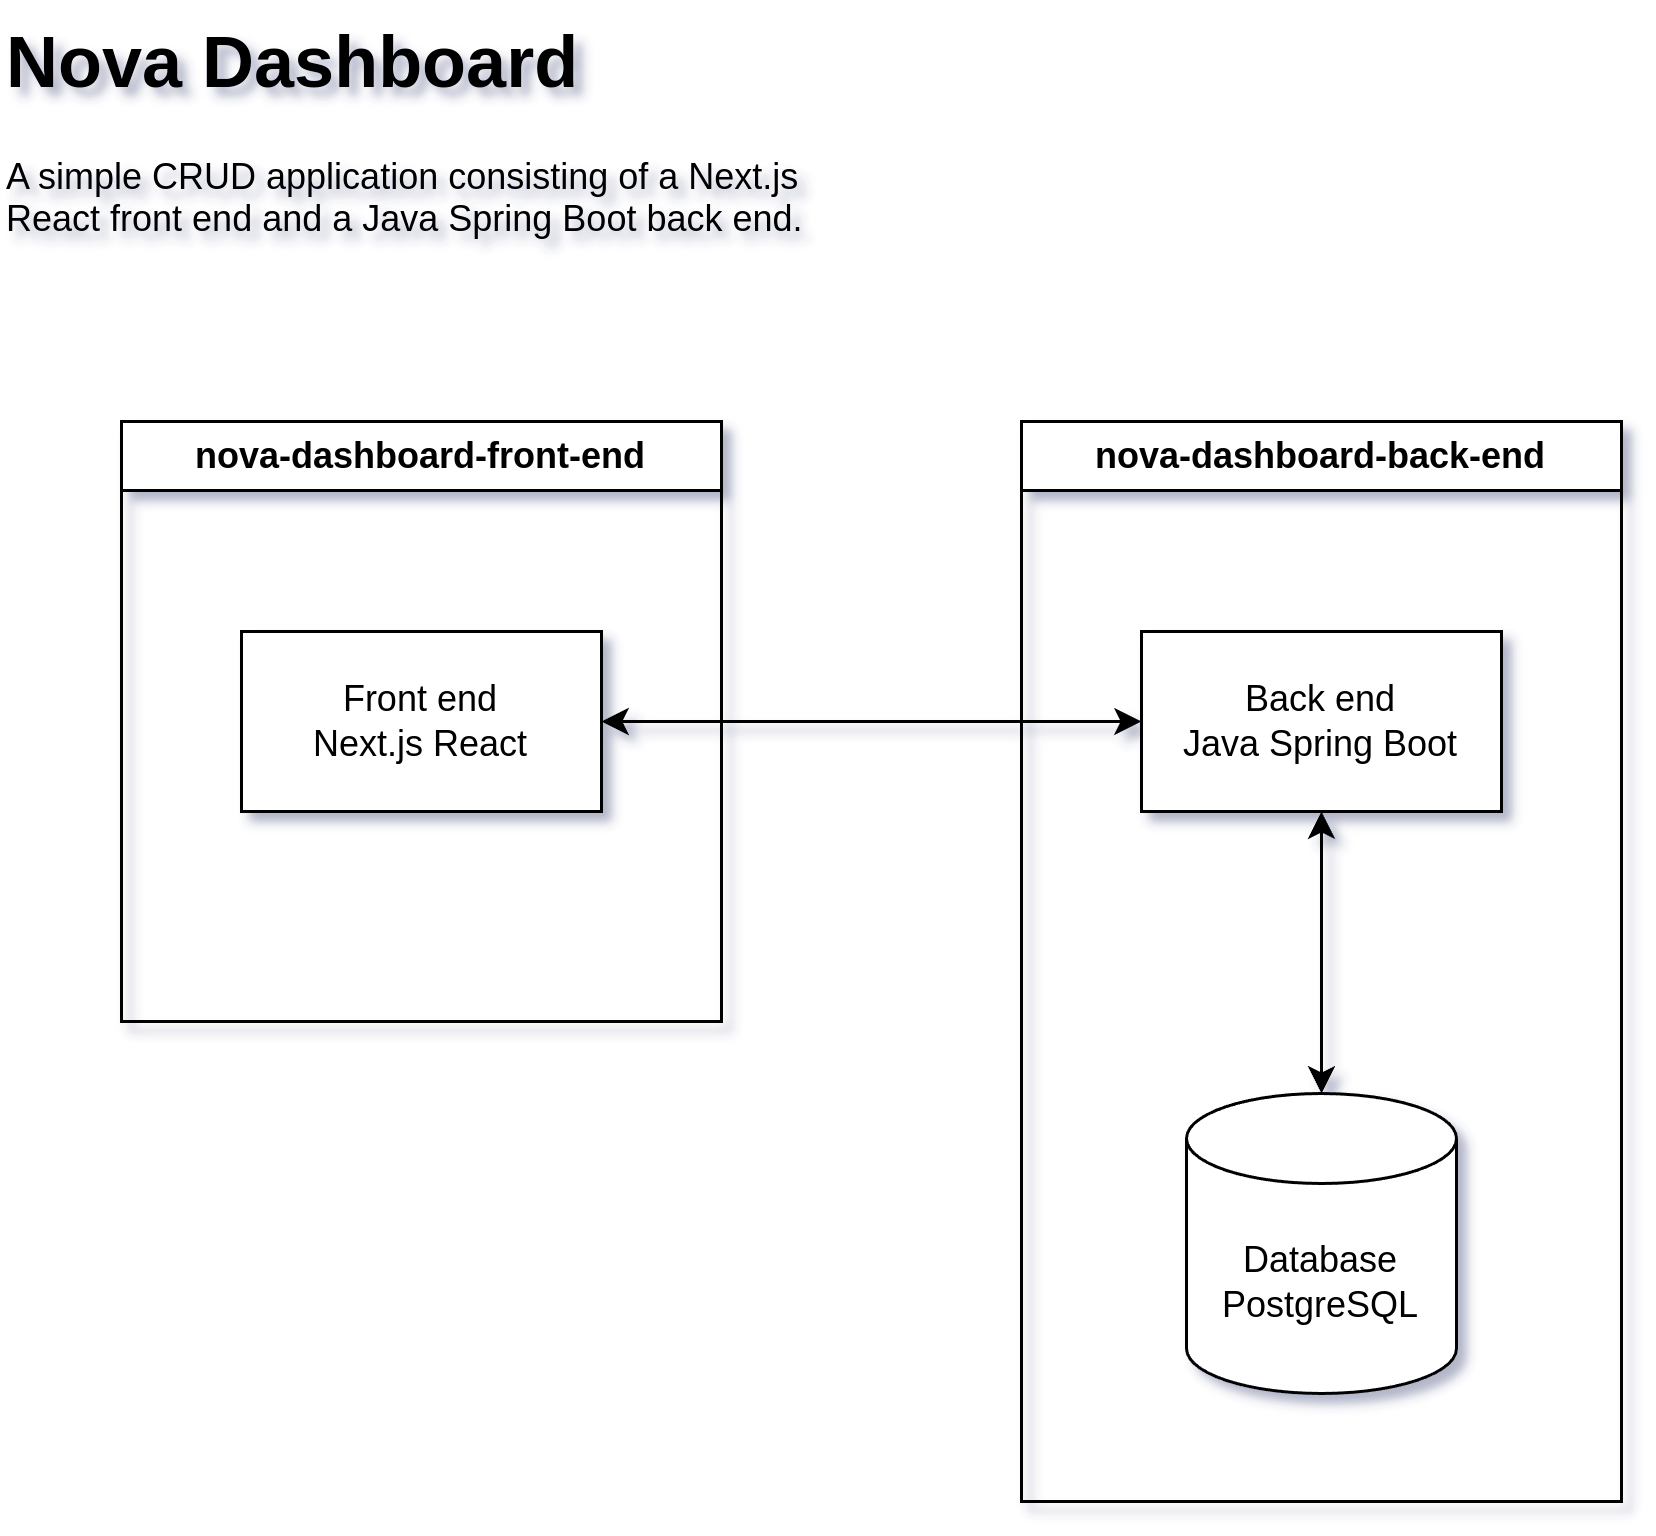
\includegraphics[width=.5\textwidth]{architecture-overview.png}
    \caption{An overview of the system architecture.
    }\label{fig:architecture-overview}
\end{figure}

\begin{figure}[H]
    \centering
    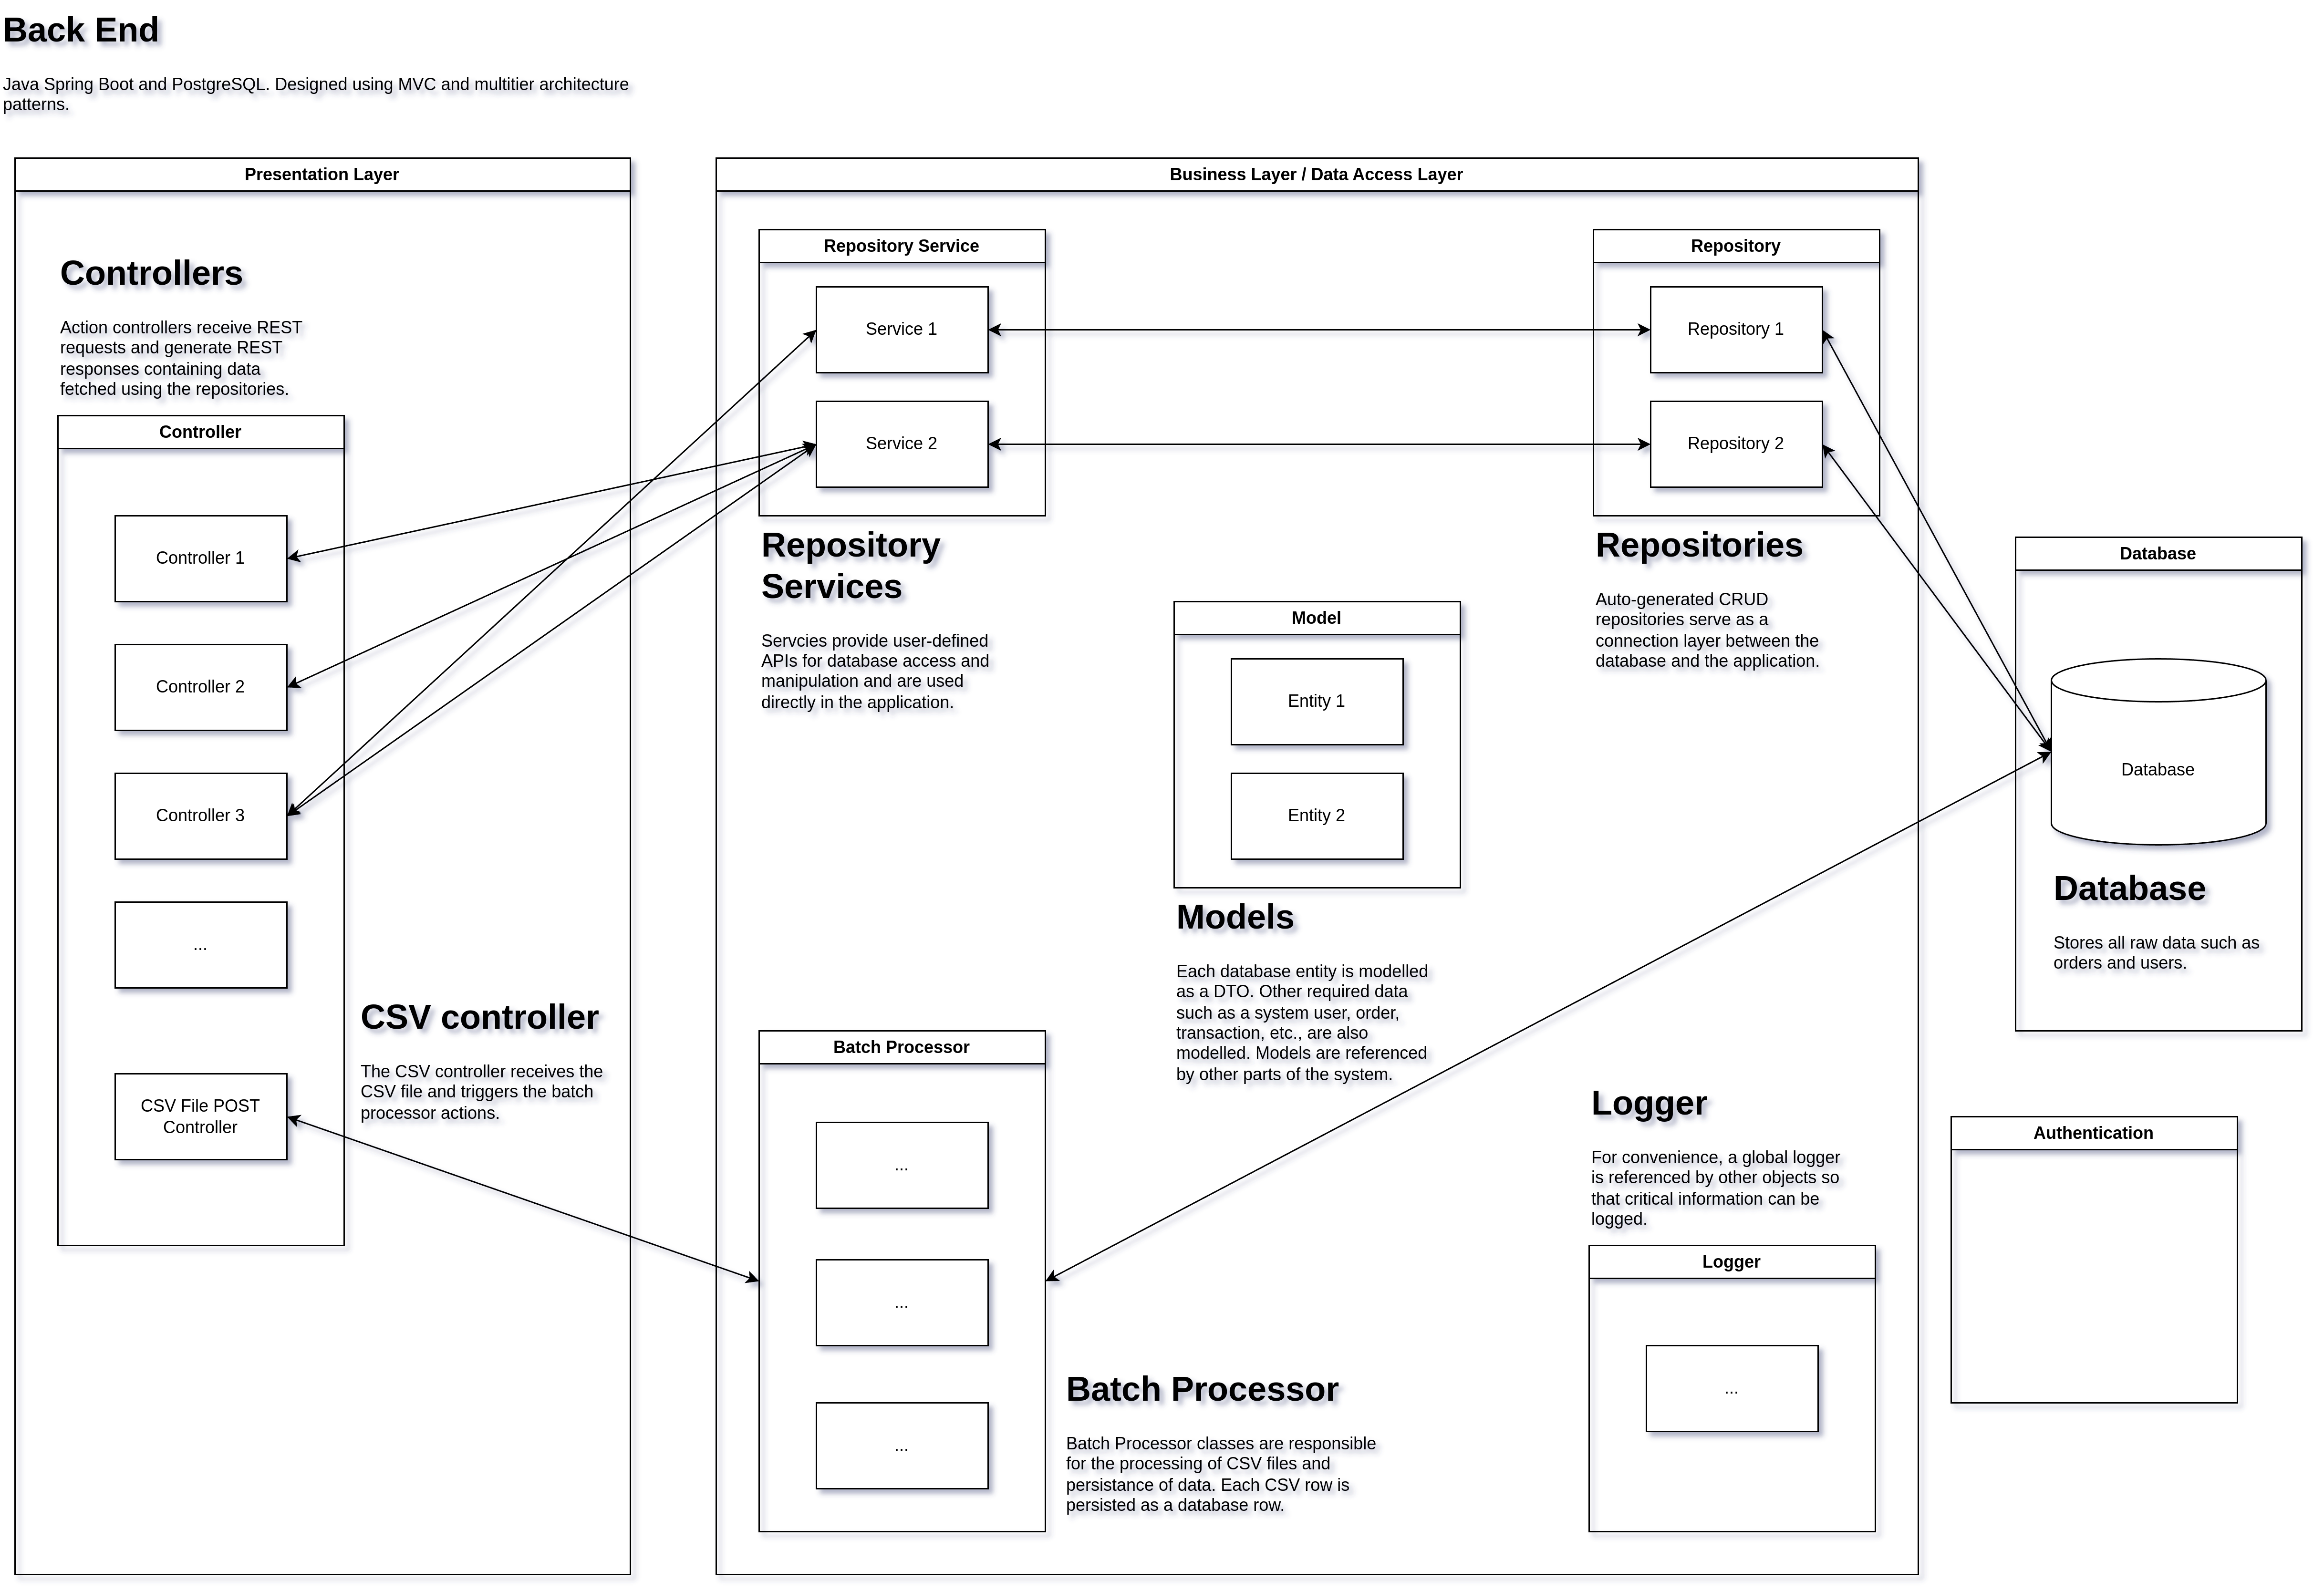
\includegraphics[width=\textwidth]{architecture-backend.png}
    \caption{The back end architecture.
    }\label{fig:architecture-backend}
\end{figure}

The diagram in Figure~\ref{fig:architecture-overview} shows a top-level overview of the system architecture.
It shows how the system is divided into two different development environments, a front end and a back end.
The front end is using~\url{Next.js}, which is a framework for React.
The back end is using Java with Spring Boot.
It is also connected to a PostgreSQL database.

The diagram in Figure~\ref{fig:architecture-backend} shows the back-end architecture.
It is a lot more detailed than the top-level overview.
The back end is split in a business layer and a data access layer.
The business layer is where the controllers are located.
The controllers are responsible for handling the requests from the front end using the REST API.\@
One special controller is the ``CSV File POST'' controller, which is responsible for handling the CSV files that
are uploaded to the system from the front end.
This is necessary to handle the sales data from the~\acrshort{epos} system.
That controller is connected to a batch processor in the data access layer.
The batch processor is responsible for processing the CSV files from comma separated values to database entries.
By utilizing a batch processor, the system can handle large amounts of data without compromising performance.
The other controllers are connected to repositories in the data access layer.
These repositories are responsible for handling the database queries.
Lastly, the data access layer also contains models for the database entries and a logger for logging errors.
Both the batch processor and the repositories are connected directly to the database.
The batch processor is inputting data into the database, while the repositories are querying the database for data.
This keeps the database secure and reliable.
